%----------------------------------------------------------------------------
\chapter{Graph schema and generation}
%----------------------------------------------------------------------------

This chapter covers the initial technical setup and data generator specification which  will be used to seed graph database.
The same schema and graph instances are used in all database systems.
The schema describes all node labels, properties, and edge types among them.
As financial institutions are isolated for privacy concerns and do not provide data for research purposes, in this work, a synthetic data generator is developed to provide regular and fraudulent transaction datasets.

%----------------------------------------------------------------------------
\section{Graph schema}
%----------------------------------------------------------------------------

A graph schema has been designed to eliminate the memory redundancy in all fraud scenarios.
There are three vertex labels and four edge relationships, as illustrated in \autoref{fig:schema}.

\begin{itemize}
    \item {Vertices}
    \begin{enumerate}
        \item \textbf{User} defines a label for customers of a banking or an e-commerce platform
        \item \textbf{Good} contains basic properties of online selling products 
        \item \textbf{Merchant} describes the product owners in an e-commerce platform
    \end{enumerate} 
    
    \item {Edges}
    \begin{enumerate}
        \item \textbf{Connection} maps the friendship relations among users
        \item \textbf{Transaction} illustrates the money transfer between two bank accounts
        \item \textbf{Review} contains the review rating of a product by a customer in an e-commerce platform
        \item \textbf{Ownership} defines a simple relationship between product and merchant
    \end{enumerate}
\end{itemize}

The user label is used in all scenarios and has the most relationship connections, among others.
On the other hand, good and merchant labels are only used in biased review scenarios.
Users can have transaction and connection edges among themselves and only review type with goods.

Only a merchant can own a good, and the ownership relationship between them doesn't have a timestamp property.
In the current implementation of the experiments, the timestamp property of edge connections is not used for queries.
However, in the next phase, the real-time data seeding will be integrated, and frequency-based processing will be included in the monitoring system.

\begin{figure}[!ht]
    \centering
    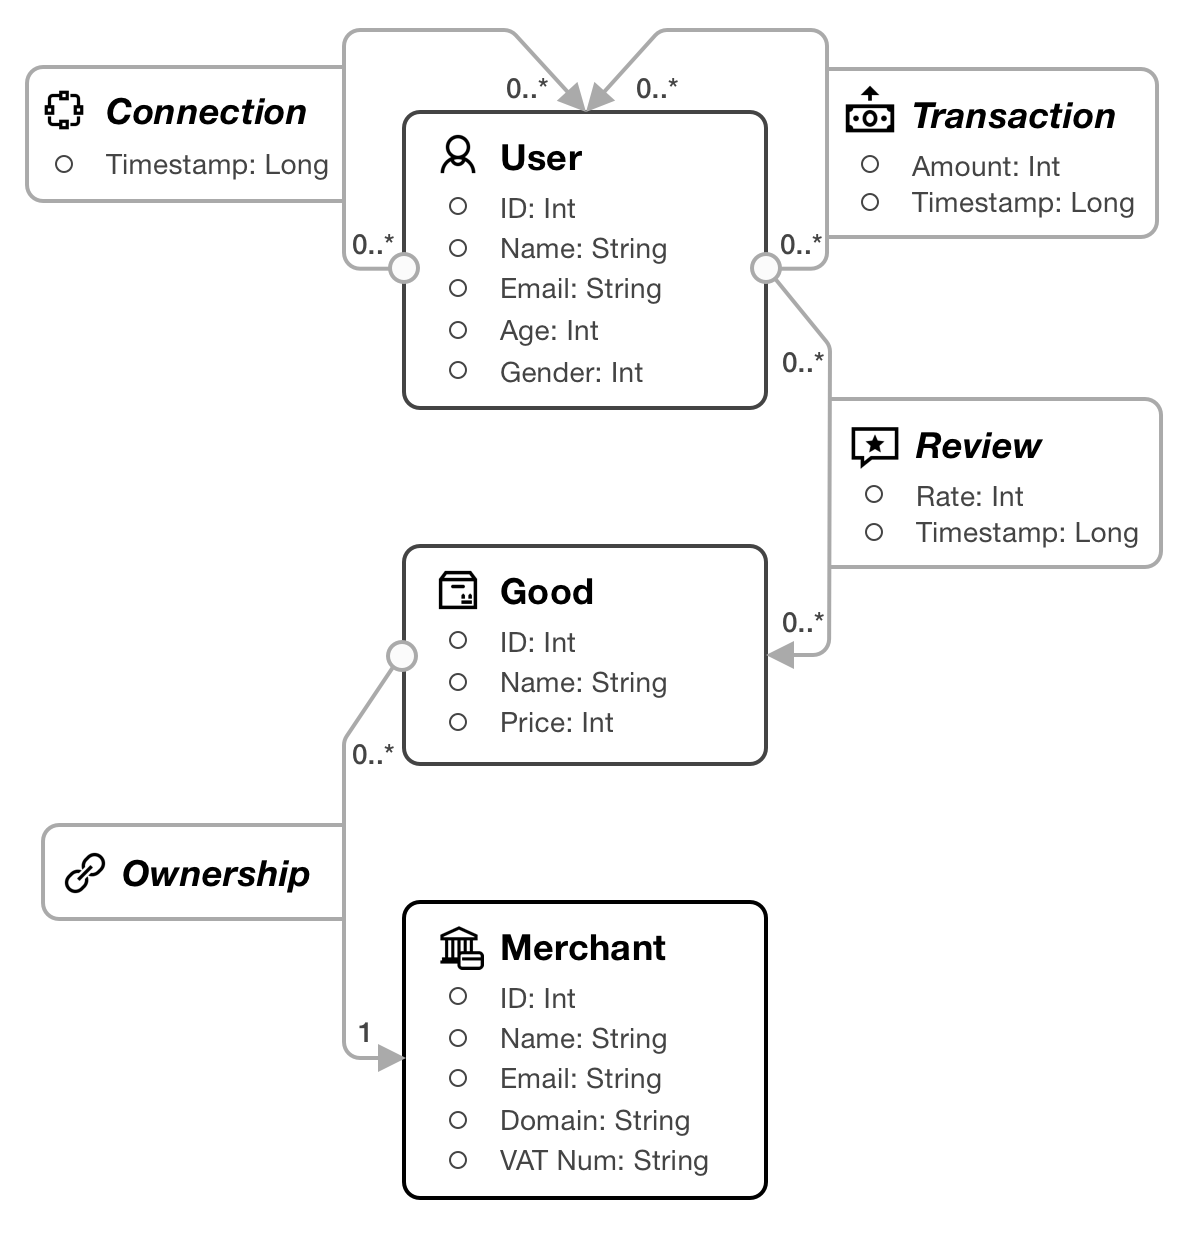
\includegraphics[scale=0.3]{figures/schema.png}
    \caption{Graph schema} 
    \label{fig:schema}
\end{figure}

%----------------------------------------------------------------------------
\section{Synthetic data generator} \label{sec:syntetic_data_generator}
%----------------------------------------------------------------------------

A Java console application is developed to generate synthetic datasets for the system and is available publicly in a GitHub repository\footnote{\url{https://github.com/kerimovscreations/cardfrauddatagen}}.
To generate meaningful and a wide variety of random data for vertices \textbf{jFairy}\footnote{\url{https://github.com/Devskiller/jfairy}} Java library is used.
The library is used to generate fake user and merchant details.

In addition, the distribution of transaction amount is normalized with another Java library called \textbf{MockNeat}\footnote{\url{https://github.com/nomemory/mockneat}}.
The probability distribution of transaction amounts is divided into three range respectively, \$0--100 (50\%), \$100--300 (30\%), \$300--500 (20\%).
The library is also used to generate the names (nouns) for the goods' name property.

The application contains two kinds of generators, standard and fraudulent injector.
Datasets of fraudulent data injectors are also used to verify the graph query results.

\begin{itemize}
    \item General data generators (based on the graph schema)
    \begin{enumerate}
        \item Vertices
        \item Edges
    \end{enumerate}
    \item Fradulent data injectors
    \begin{enumerate}
        \item Smurfing -- distributed, then centralized transactions. 
        The generator picks random sender and receiver user ids, then generates the transactions chain through 3 to 10 middleman accounts.
        \item Cyclic transactions. The injector generates an open loop transactions chain through middleman accounts, and a friendship relationship to close the loop. 
        \item Biased reviews. The injector picks a random merchant, then assigns ownership relationships of 5--10 goods. At the next step, it picks random 2--5 users and assigns 5-star reviews from these users to the goods picked before.
    \end{enumerate}
\end{itemize}

The generator has two output size configurations: small and large datasets.
These configurations are designed to generate 50K vertices with 100K edges and 500K vertices with 1.2M edges, respectively (\autoref{fig:dataset_sizes}).

\begin{figure}[!ht]
    \centering
    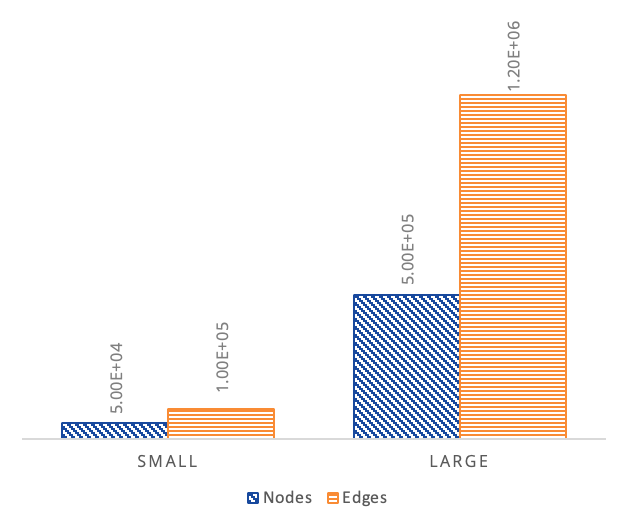
\includegraphics[width=0.6\textwidth]{figures/dataset_sizes.png}
    \caption{Comparison of dataset sizes} 
    \label{fig:dataset_sizes}
\end{figure}

